We begin with an illustrative synthetic case study chosen to highlight the trade-offs that decision-aware training allows a modeler to make when working with misspecified models. 

\begin{figure*}[!t]
\begin{tabular}{c c}
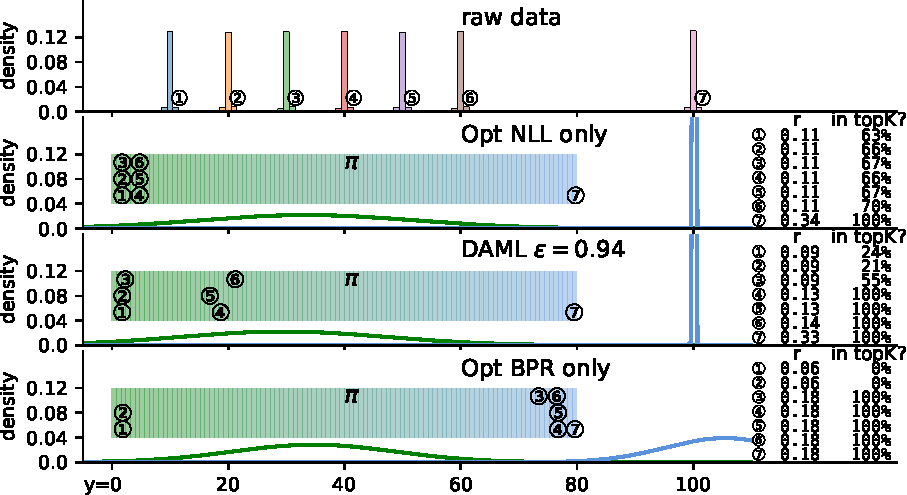
\includegraphics[width=.6\textwidth]{figures/synth1D_data_and_models.pdf}
&
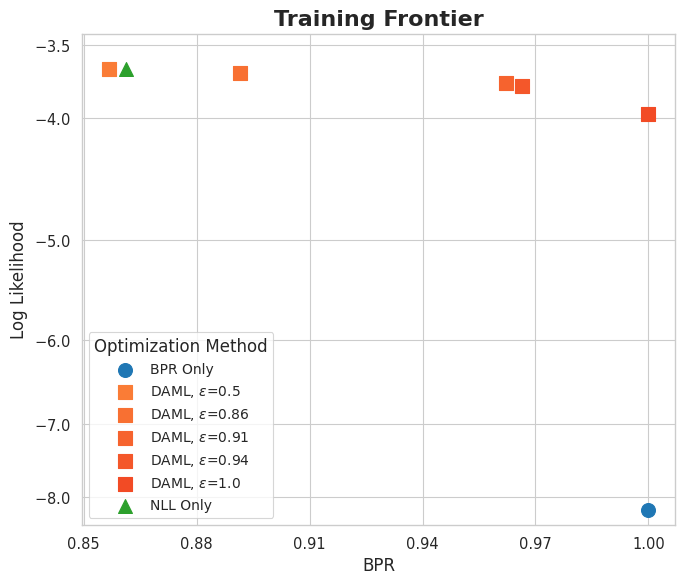
\includegraphics[width=.35\textwidth]{figures/SynthFrontierSquare.png}
\end{tabular}
\captionof{figure}[Synthetic 1D data: learned models and Pareto frontier.]{
\textbf{Synthetic 1D data: learned models and Pareto frontier.} \textit{Left Row 1:} histograms of $y_s$ values by site (circled numbers). Sites 3-7 should be the top K=5 under the true model.
\textit{Left Rows 2-4:} Learned Gaussian components, with site-specific weights $\bm{\pi}_s$ marked as horizontal position between pure green and blue. Text provides ranking $r$ with how often that site is in top $K=5$ over 200 trials.
\textit{Right:} Likelihood vs. BPR tradeoff frontier for final models delivered by different training objectives.
% performance of models trained with differing objectives. In the top-left corner, we see models trained purely to maximize log-likelihood obtain the highest likelihood and lowest BPR-5. This is caused by the underlying model being a mixture of 2 components. To maximize likelihood, the 6 low-valued locations are grouped together, and the 1 high-value location recieves its own component. Conversely, models trained to maximize BPR alone are in the lower-right corner of the graph, with perfect BPR and the lowest likelihood. This is caused by the model choosing 1 component containing the 5-largest locations, and spanning the large gap between 60 and 100. In between these two extremes, our new hybrid objective allows for finding the highest-likelihood model which satisfies a given BPR threshold.
}%end caption
\label{fig:synth_data_and_results}
\end{figure*}

\textbf{Task.} We create a synthetic dataset of $S=7$ sites over $T=500$ times. Integer data $y_{ts}$ is generated i.i.d over time from a quantized Gaussian with site-specific mean and small constant variance. The first six sites have means evenly spaced between 10 and 60; the last site has a large mean of 100. Fig.~\ref{fig:synth_data_and_results} (top left) shows the training data.

\textbf{Model.} To show the benefits of our framework, we focus on a \emph{misspecified model}. In particular, we model each site with a $L$-component positive Gaussian mixture model, with global mean and variance parameters and site-specific component frequencies:
\begin{align}
    p_{\phi}(y_s) &= 
    \textstyle \sum_{\ell=1}^L \pi_{s,\ell} \cdot \mathcal{N}_+(y_s|\mu_\ell, \sigma_\ell^2)
    \label{eq:model}
\end{align}
Here $\phi = \{ \mu_{1:L}, \sigma_{1:L}, \pi_{1:S,1:L} \}$. 
We reparameterize to unconstrained real values to make gradient-based learning possible: see App.~\ref{supp:synth1D} for details.

With $L{=}7$ components, the model would be well-specified and could recover the true data-generating process. However, we focus on misspecification, so we fit with $L{=}2$ components. This will hurt likelihood performance, as sites with distinct true means will need to use common means. However, we wish to show that solid top-K decision-making can still happen even with such severe misspecification.

\textbf{Experiment setup.} We use BPR with $K=5$ for this task. 
For reproducible details, including all hyperparameters, see App.~\ref{supp:synth1D}.
We only report training set metrics here for simplicity; later tasks assess generalization to test data.

%The modeling goal is to learn $\phi$ that yields the best where-to-intervene decisions in terms of BPR when K=5, while also delivering high likelihood. We compare all three approaches from Sec.~\ref{sec:methods_train}: ML estimation, direct minimization of BPR, and DAML.

%We train a spectrum of 7 models, all with gradient descent. One optimizes purely the ML objective. Another optimizes the BPR loss alone. The 5 intermediate models use our DAML objective with different $\epsilon$ values to enforce different constraints on BPR, intending to sweep out intermediate points on the two-objective Pareto frontier.
%For each model, we run 20 random initializations to convergence each with 3 possible learning rates. We keep the $\phi$ estimated by the single run that best optimized the model's objective. Using multiple initializations helps avoid the local optima common to mixture models.

%For models with BPR losses, we try perturbation noise levels of 0.01 and 0.05, use 500 samples for both Monte Carlo estimates to focus on high-quality rather than speed. For reproducible details, including all hyperparameters and algorithmic details, see Supp.~\ref{supp:synth1D}.

\textbf{Results and analysis.}
From results in Fig.~\ref{fig:synth_data_and_results}, we draw several conclusions.
First, training to optimize NLL alone delivers subpar BPR for this task, as expected. 
Second, optimizing for BPR alone yields much better BPR values, suggesting that even this mispecified model can deliver much better top-K decision making than the off-the-shelf ML solution. However, BPR alone yields nonsensical likelihood values, as nothing in the objective forces $\phi$ to be good at modeling the outcomes $y$, only at relative ranking of the $S$ sites.
In Fig.~\ref{fig:synth_data_and_results}, we see how our DAML hybrid objective allows a user to traverse the Pareto frontier of likelihood and BPR by enforcing a desired threshold on minimum BPR. As the desired minimum BPR threshold $\epsilon$ increases, we can sweep the tradeoff between likelihood and BPR. Ultimately, our DAML yields the best high-likelihood, high-BPR solutions in the top-right corner of the Pareto plot.


%We see that by using the decision-aware training objective, we can maximize BPR while still obtaining a highly likely model.


% is given 20 random initializations of the model parameters. We use a learning step-size of 0.1. For models with BPR in the objective, we try a perturbation noise of both 0.01 and 0.05, with 500 samples. In the hybrid models, we use $\lambda=30$, selected so that the likelihood term and the BPR penalty term are on the same order of magnitude after several epochs of training.

% of 7 simulated locations. Each location has an observable quantity that is sampled from a distribution that is stationary in time. We model the $S=7$ dimensional vector $y_t \in \mathbb{R}^{S}$. We wish to take the best action to reach $K=5$ locations. 

%At each location, the outcome at each time is drawn from a normal distribution with small variance. One of the locations has a relatively large mean value of 100. The mean values of the other six locations are evenly spaced between 10 and 60. We sample 500 observations from each location to make our dataset. An illustration of the the data is shown in Figure \ref{fig:synth_data}.


% \subsubsection{Misspecified model}
% We will sample data from these synthetic locations, and build models that attempt to maximize BPR using the three approaches from Section \ref{section:training}: ML estimation, Direct loss minimization,  and Decision-constrained maximum likelihood training.

% It is important here to consider models that are misspecified. For this synthetic example where we have full knowledge and control of the data generating process, it would be trivial to use a well-specified model that could obtain the optimal likelihood and BPR for decision making. However, in real-world scenarios our models are almost always misspecified in some way.

